\chapter{Geheugenarchitectuur}
\label{architecture}
Om overzicht te houden op de geheugenarchitectuur, zijn bepaalde bouwblokken gedefinieerd. Het grootste bouwblok is de global block, dit bestaat uit twee local blocks en een sense amplifier. Local blocks zijn geheugencelmatrices met decoders en passgates er rond.
Dit hoofdstuk bespreekt de algemene structuur alsook de vrijheidsgraden die in hoofdstuk \ref{timing-optimization} onderzocht worden om tot een optimaal werkend systeem te komen. Ten slotte zullen ook nog de bouwblokken vermeld worden die meer uitvoerig besproken worden in de volgende hoofdstukken. 


\section{Cel}
Dit elementaire bouwblok is besproken in sectie \ref{1T1R} en vormt de kern van het geheugensysteem.
De cel bestaat uit een memristor en een transistor (1T1R-cel). De geheugencel heeft drie terminals: de gate van de transistor, die verbonden wordt met een wordline, de source van de transistor, die verbonden wordt met een sourceline en tenslotte de terminal van de memristor, die verbonden wordt met een bitline.
%Een cel waarvan memristor zich in een willekeurige resistieve staat bevindt is een datacel, terwijl de memristor van referentiecellen in een voorgeprogrammeerde en dus gekende resistieve staat verkeert.

\section{Branch}
De branch en cel worden getoond in figuur \ref{fig:cellbranch}. In een branch worden er een bepaald aantal datacellen verbonden aan één BL en één SL. Dit aantal wordt \emph{Number of Word Lines per Branch} (NoWLpB) genoemd en is een van de vrijheidsgraden van deze geheugenarchitectuur. Naast alle datacellen is er ook nog één referentiecel - dit is een cel waarvan de resistieve staat voorgeschreven is - verbonden aan de BL en SL van de branch.
Elke BL wordt via een pMOS-transistor (al dan niet met nog een impedantie tussenin) gekoppeld aan de voedingsspanning Vdd en via een nMOS-transistor aan de grondspanning Vss. In dit werk is er enkel een nMOS-transistor die de SL verbindt met Vss.\footnote{In een volledig geheugensysteem zou de SL via een pMOS ook nog verbonden zijn met een niet onderzochte spanningsknoop Vdd\_write. De pMOS zou dan worden aangezet voor schrijfwerking.} De nMOS-transistoren aan BL en SL fungeren als schakelaars, de pMOS-transistor wordt daarenboven ook gebruikt als impedantie voor een resistieve spanningsdeling (zie hoofdstuk \ref{loadanalysis}).

\begin{figure}
  \centering
  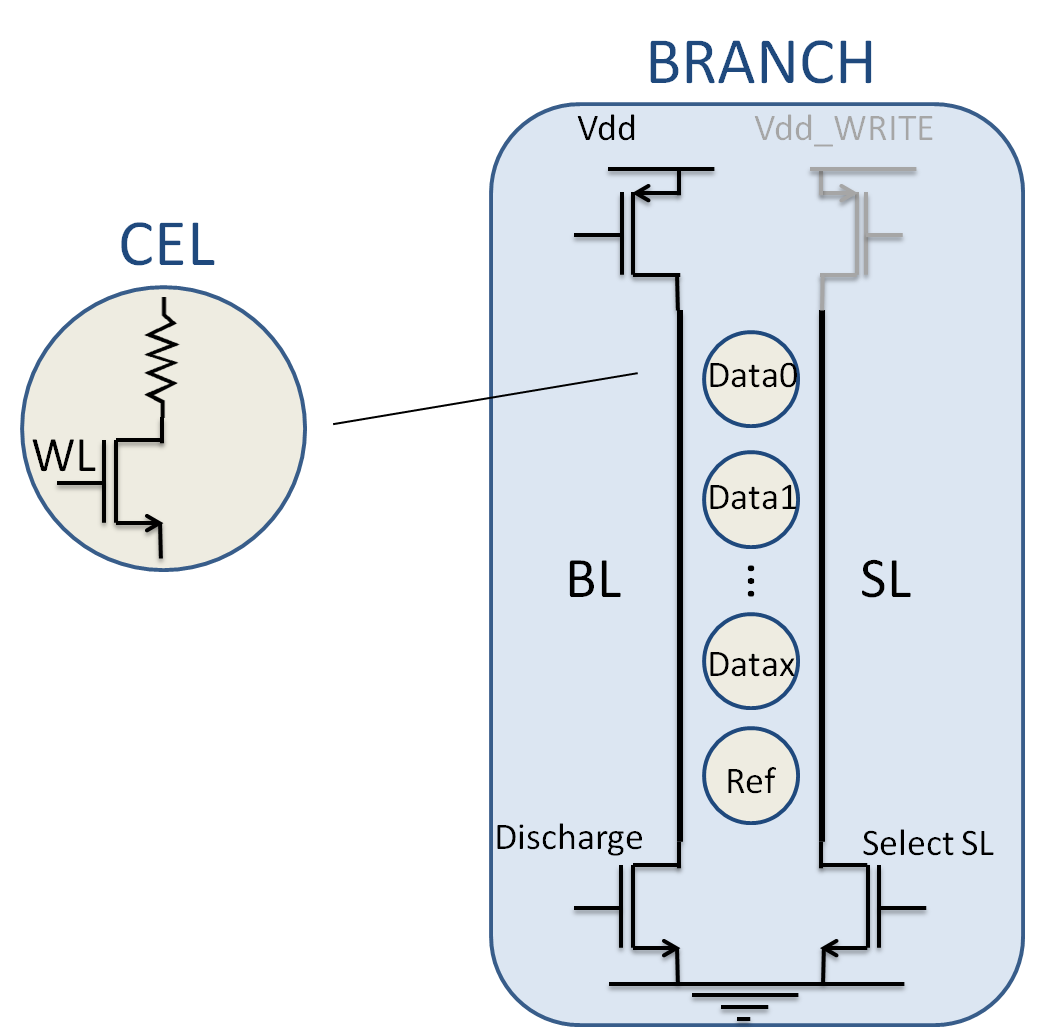
\includegraphics[scale=0.3]{../fig/hfdstk-architecture-cell-branch.png}
  \caption[Een geheugencel en een branch]{Een geheugencel en een branch}
  \label{fig:cellbranch}
\end{figure}

\section{Local Block}
Verschillende BLs en SLs worden samengebracht in een local block, waarvan de vrijheidsgraad \emph{Number of BitLines per Local Block} (NoBLpLB) heet. In een LB bevinden er zich dus NoBLpLB x NoWLpB datacellen en NoBLpLB referentiecellen. Ook bevat een local block zowel BL- als WL-decoders. De afzonderlijke BLs worden via passgates verbonden tot een uitgangsknooppunt.
De structuur van een local block wordt afgebeeld op figuur \ref{fig:LB}, een meer gedetailleerd beeld - zonder decoders - is getoond op figuur \ref{fig:LB-details}.
De uitgangen van de WL-decoder sturen de data-WLs aan [eventueel met een buffer], de uitgangen van de BL-decoder activeren een spanningsdeling op de BLs.\footnote{Indien schrijfbewerking zou toegevoegd worden, zouden de uitgangen van de BL-decoder aan twee AND-poorten worden verbonden; bij leesoperatie brengt de uitgang van de ene AND-poort de resistieve deling op de BL teweeg, bij schrijfoperatie zet de uitgang van de andere AND-poort een pull-up-operatie van de BL naar Vdd\_write op.} De referentie-WL is via een extern signaal verbonden. Voor een gedetailleerdere beschrijving over hoe de decoderuitgangen gebruikt worden, zie sectie \ref{timing}.
Een LB heeft twee werkingsmodes: een mode waarbij er één datacel wordt aangesproken om een datasignaal aan de uitgang te verkrijgen en een mode waarbij er een bepaald aantal referentiecellen in parallel wordt aangesproken om een referentiesignaal aan de uitgang te verkrijgen.

\begin{figure}
  \centering
  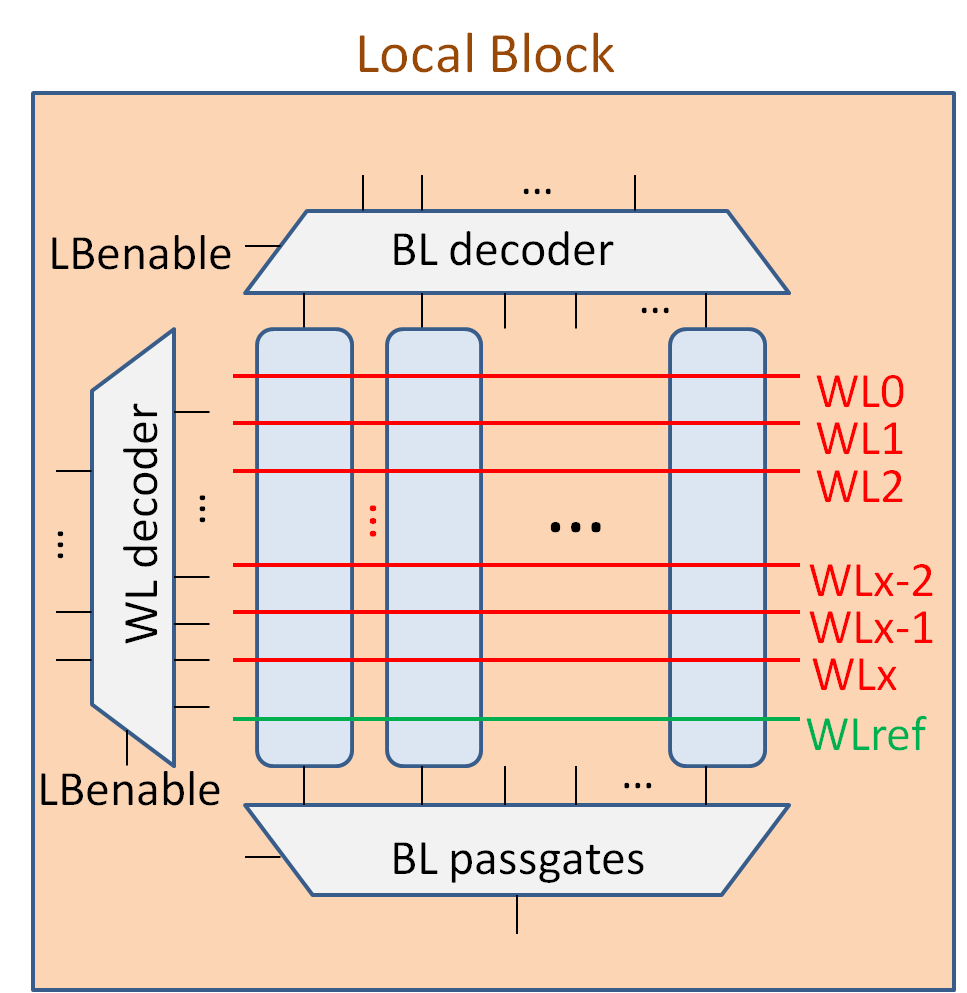
\includegraphics[scale=0.3]{../fig/hfdstk-architecture-localblock.png}
  \caption[Een local block]{Een Local Block}
  \label{fig:LB}
\end{figure}

\begin{figure}
  \centering
  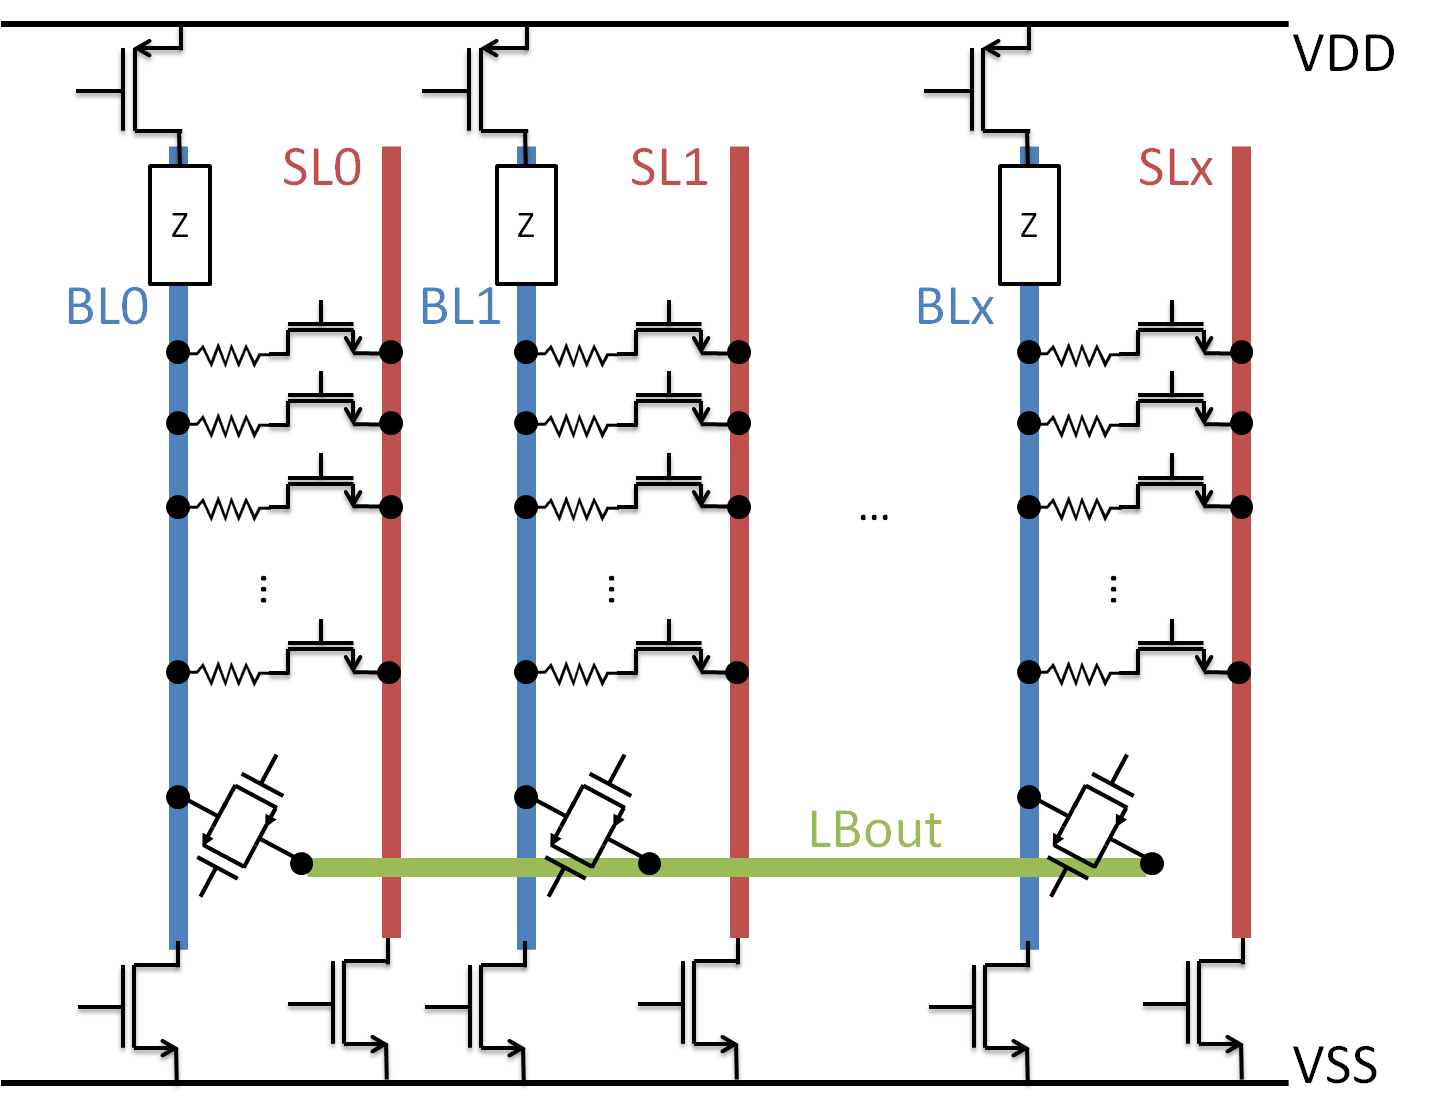
\includegraphics[scale=0.3]{../fig/hfdstk-architecture-LB-details.png}
  \caption[Een local block]{Een meer gedetailleerde illustratie van een LB, decoders zijn weggelaten}
  \label{fig:LB-details}
\end{figure}

\subsection{Dataspanning genereren uit datacel}
\label{dataread}
Het datasignaal is de spanning op de BL wanneer er een resistieve deling aan de gang is, waarbij er stroom vloeit door één cel. De last die hangt aan de voedingsspanning, op figuur \ref{fig:dataread} voorgesteld als een pMOS-transistor en optionele extra impedantie, wordt aangeschakeld, alsook de nMOS-transistoren in de cel en aan de sourceline. Deze vormen met de weerstand van het geheugenelement zelf de equivalente totale weerstand Rtot. Er vloeit een stroom langs dit pad: I=Vdd/Rtot en de spanning op de BL is V=IReq met Req de equivalente weerstand van de SL-transistor- en celimpedantie. Om dit datasignaal op de uitgangsknoop van het LB te krijgen, wordt de bijhorende passgate van de BL in kwestie geactiveerd.

\begin{figure}
  \centering
  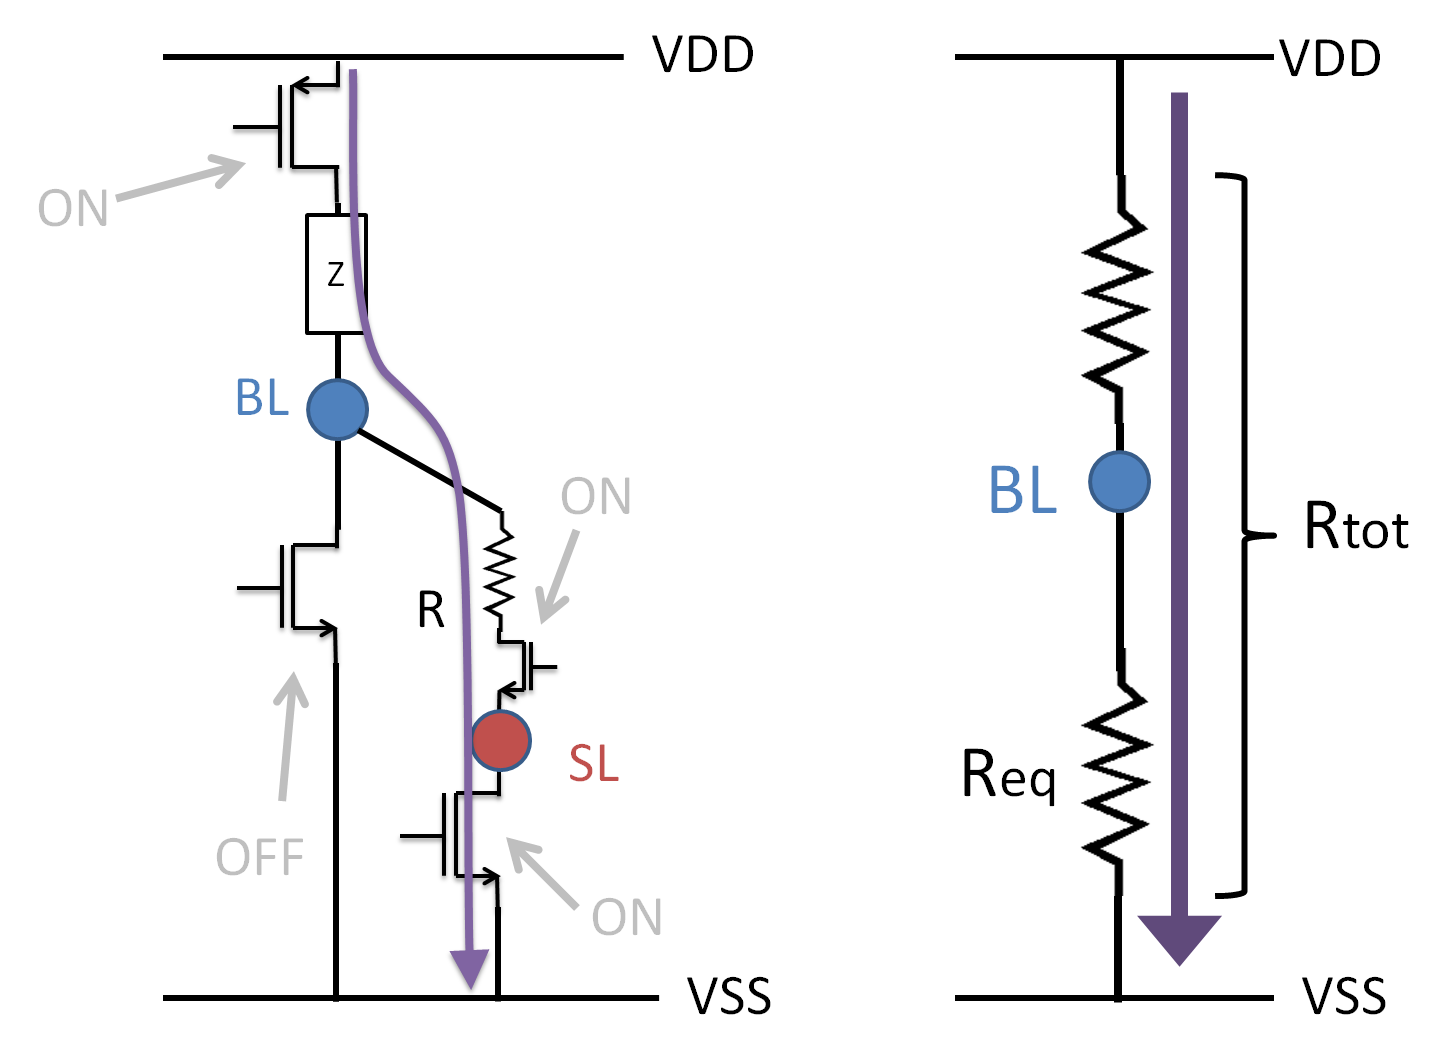
\includegraphics[scale=0.3]{../fig/hfdstk-architecture-datasignal.png}
  \caption[Datasignaal uitlezen]{Spanningsdeling waarbij dataspanning over BL staat}
  \label{fig:dataread}
\end{figure}

\subsection{Referentiespanning genereren uit referentiecellen}
\label{refread}
Het referentiesignaal is een spanning die tussen de spanning van een LRS datasignaal en een HRS datasignaal moet liggen. Een dergelijk signaal kan verkregen worden door twee BLs kort te sluiten zoals op figuur \ref{fig:2cellref}. In dit ontwerp zal de kortsluiting gerealiseerd worden door de passgates van de BLs aan te zetten, zo komt het referentiesignaal bovendien ook op de uitgangsknoop te staan. In theorie is het voldoende om 2 BLs [de ene met een HRS cel en de andere met een LRS cel] kort te sluiten om het referentiesignaal te verkrijgen. Er zit echter op de resistieve geheugenelementen variabiliteit: er wordt aangenomen dat $R_{H}$ normaal verdeeld is met $\mu = 32500\Omega$ en $\sigma = 833\Omega$. $R_{L}$ is ook normaal verdeeld met $\mu = 7500\Omega$ en $\sigma = 833\Omega$. Dit betekent dat ook de data-signalen en referentie-signalen stochastische variabelen zijn.
Door meerdere referentiebitlijnen kort te sluiten gaat de spreiding van het referentiesignaal dalen [maar het energieverbruik stijgen]. Bovendien kan men de verwachtingswaarde verschuiven door meer HRS (LRS) referentiegeheugenelementen te gebruiken dan LRS (HRS).

\begin{figure}
  \centering
  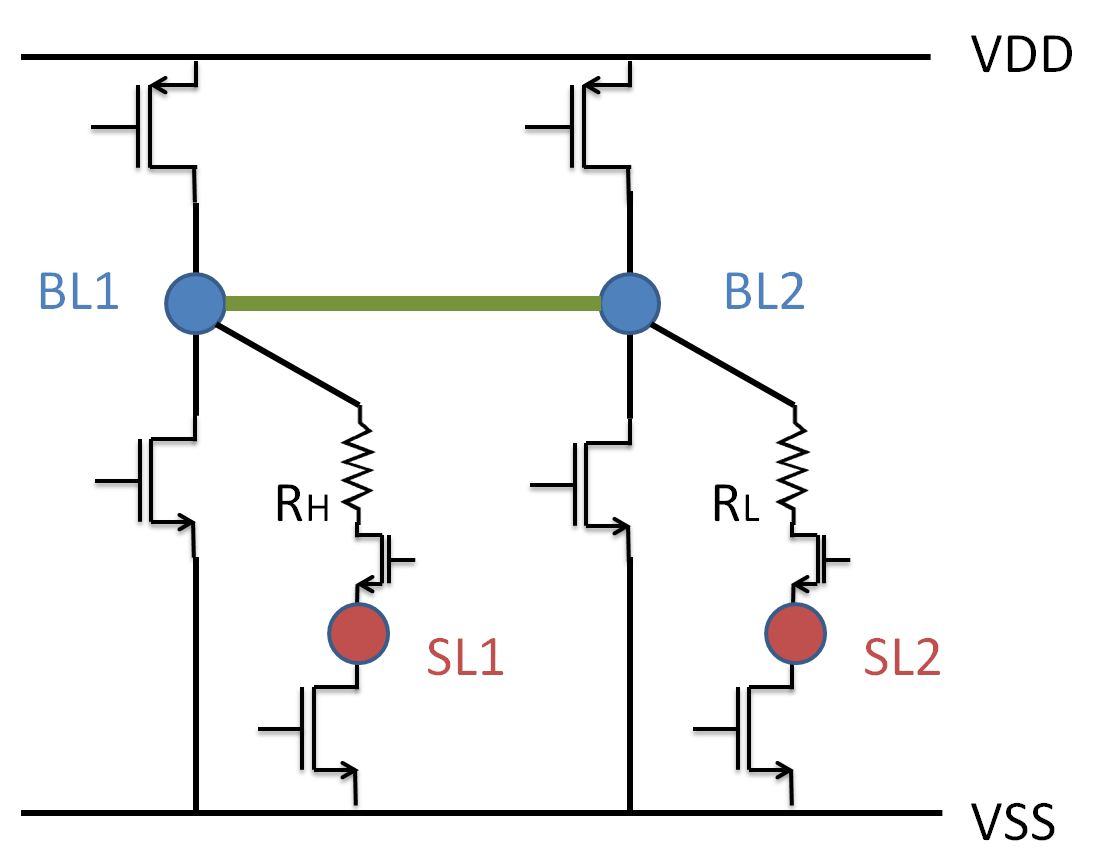
\includegraphics[scale=0.3]{../fig/hfdstk-architecture-ref2cell.png}
  \caption[Referentiesignaal uitlezen]{Topologie om referentiesignaal te verkrijgen}
  \label{fig:2cellref}
\end{figure}

\section{Global Block}
\label{globalblock}
Een global block bestaat uit twee LBs en een sense amplifier (SA) met bijhorende sample-and-hold-schakelaars (S\&H). De S\&H-schakelaars worden geïmplementeerd met passgates. In het ene LB gaat er een datasignaal geproduceerd worden, in het andere een referentiesignaal (zie figuur \ref{fig:GB}). Vervolgens gaat de SA dit kleine signaalverschil versterken tot een zuivere rail-to-rail output.
Aan de uitgang van het GB verschijnen dan ook de opgevraagde bits.
De laatste architectuurvrijheidsgraad is de \emph{Number of Global Blocks} (NoGB), het totale geheugen bevat NoGB x 2 x NoBLpLB x NoWLpB datageheugencellen.



\begin{figure}
  \centering
  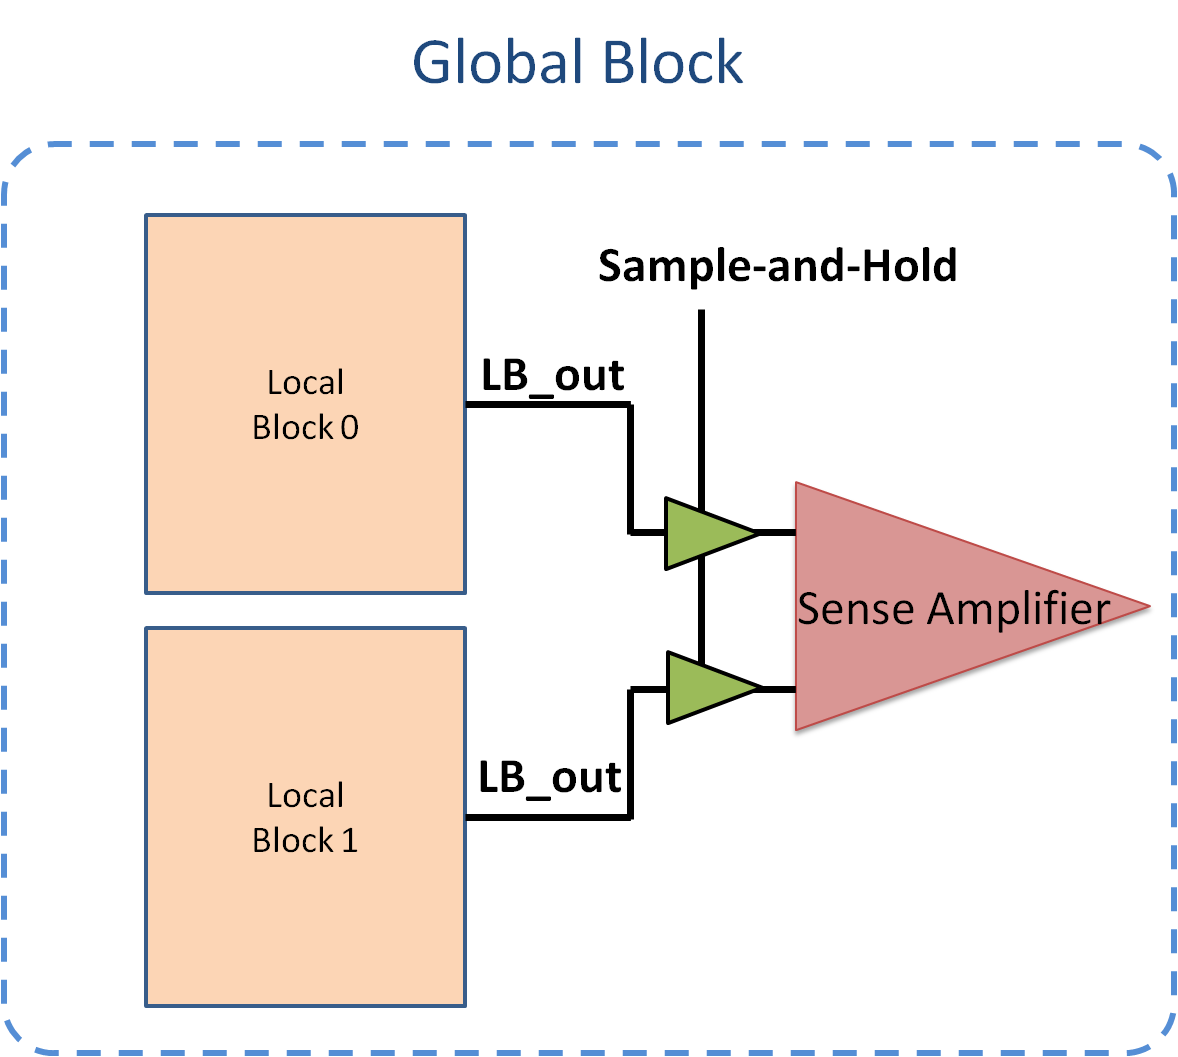
\includegraphics[scale=0.3]{../fig/hfdstk-architecture-globalblock.png}
  \caption[Een global block]{Een global block}
  \label{fig:GB}
\end{figure}

\section{Besluit}
De geheugenarchitectuur werd in vogelvlucht overlopen. Het kleinste bouwblok is de cel, deze wordt geplaatst in een branch, d.i. een combinatie van cellen aan een BL en SL, verbonden met schakelaars en impedanties aan VDD en VSS. Verschillende branches vormen samen met decoders en passgates een local block. Twee local blocks en een sense amplifier met bijhorende passgates worden gegroepeerd tot een global block. Het totale geheugen bestaat tenslotte uit een verzameling global blocks.

